\documentclass[a4paper,notitlepage]{article}
\usepackage[utf8]{inputenc}
\usepackage[T1]{fontenc}
\usepackage[english]{babel}
\usepackage{amsfonts,amsmath,amssymb,amsthm,graphicx}
\usepackage[pdftex,hidelinks]{hyperref}
\usepackage{tikz}
\usetikzlibrary{arrows,shapes,automata,petri}

\usepackage{enumerate}
\usepackage{verbatim}
\usepackage{csquotes}
\usepackage{cite}
\usepackage{algorithm}
%\usepackage{algorithmic}
\usepackage{algpseudocode}

\newcommand{\HIDE}[1]{}
\newtheorem{thm}{Theorem}

\title{Distributed Systems Assignment 2\\ \large{Part 2}}
\author{John L\r{a}ng, Suravi Roy}

\begin{document}

    \maketitle
   	\begin{enumerate}[1)]
   		\item
   			The Petri net given in this question has only four reachable markings,
   			$M_1$, $M_2$, $M_3$, and $M_4$, as demonstrated in Figures \ref{fig1} and
   			\ref{fig2}. Asterisks (`*') denote enabled transitions. In the initial
   			marking, $M_1$, only the transition $t_2$ may fire, which leads the Petri
   			net into marking $M_2$. In marking $M_2$, only $t_1$ may fire, so the
   			Petri net transitions into marking $M_3$. In marking $M_3$, the only
   			enabled transition is $t_3$, which transforms the Petri net into marking
   			$M_4$. After marking $M_4$, the Petri net transitions back into marking
   			$M_1$, as $t_1$ is the only enabled transition.
   			
   			Since in every one of these four markings, there is only one enabled
   			transition, the Petri net is deterministic and the sequence of markings
   			repeats infinitely
   			\begin{align}
   			    M_1 \to M_2 \to M_3 \to M_4 \to M_1 \to ...
   			\end{align}
   			According to the English Wikipedia article on Petri nets, a Petri net is
   			$L_k$-live if and only if all of its transitions are $L_k$ live. In this
   			case, the definition of $L_3$-liveness applies to the Petri net under
   			investigation, as there is the infinite firing sequence (1) in which
   			every transition fires infinitely often.
	    	\begin{figure}
	    		\centering
   				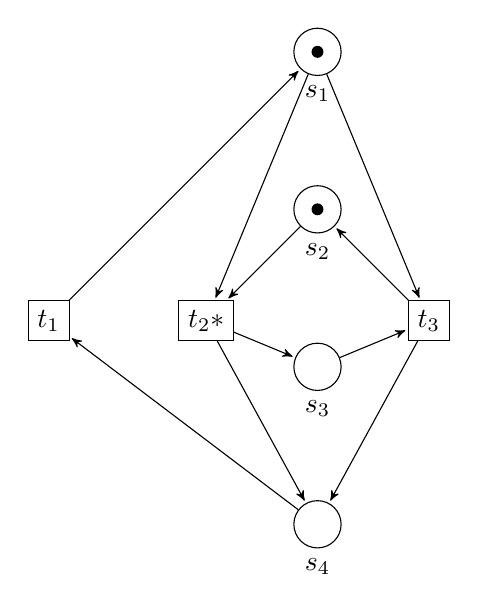
\begin{tikzpicture}[node distance=2cm,>=stealth',bend angle=45,auto]

	  				\tikzstyle{place}=[circle,draw=black,minimum size=6mm]
					\tikzstyle{transition}=[rectangle,draw=black,minimum size=4mm]
	    			\node [place,tokens=1,label=below:$s_1$] (s1) {};
   					\node [place,tokens=1,label=below:$s_2$] (s2) [below of=s1] {};
   					\node [place,label=below:$s_3$] (s3) [below of=s2]  {};
	    			\node [place,label=below:$s_4$] (s4) [below of=s3]  {};
   					\node [transition] (t2) [below left of=s2] {$t_2*$}
   						edge [pre]  (s1)
	      				edge [pre]  (s2)
   						edge [post] (s3)
   						edge [post] (s4);

	    			\node [transition] (t1) [left of=t2] {$t_1$}
  						edge [pre]  (s4)
  						edge [post] (s1);

	    			\node [transition] (t3) [below right of=s2] {$t_3$}
  						edge [pre]  (s1)
  						edge [pre]  (s3)
	     				edge [post] (s2)
  						edge [post] (s4);
				\end{tikzpicture}
				\hspace{1cm}
	    		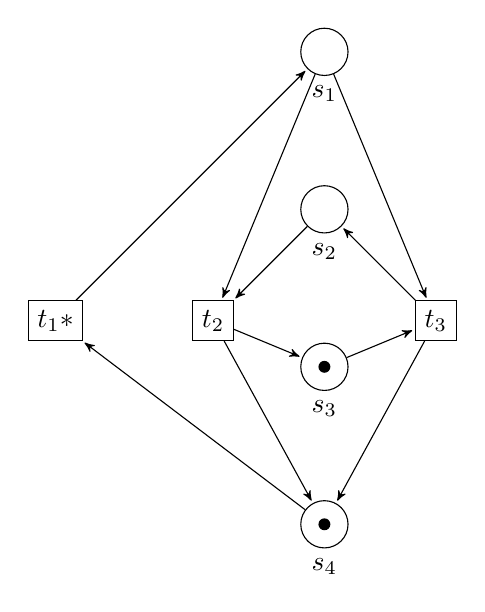
\begin{tikzpicture}[node distance=2cm,>=stealth',bend angle=45,auto]

	  				\tikzstyle{place}=[circle,draw=black,minimum size=6mm]
  					\tikzstyle{transition}=[rectangle,draw=black,minimum size=4mm]

    				\node [place,label=below:$s_1$] (s1) {};
    				\node [place,label=below:$s_2$] (s2) [below of=s1] {};
		    		\node [place,tokens=1,label=below:$s_3$] (s3) [below of=s2] {};
    				\node [place,tokens=1,label=below:$s_4$] (s4) [below of=s3] {};

    				\node [transition] (t2) [below left of=s2] {$t_2$}
		      			edge [pre]  (s1)
      					edge [pre]  (s2)
      					edge [post] (s3)
		      			edge [post] (s4);

    				\node [transition] (t1) [left of=t2] {$t_1*$}
      					edge [pre]  (s4)
		      			edge [post] (s1);

    				\node [transition] (t3) [below right of=s2] {$t_3$}
      					edge [pre]  (s1)
		      			edge [pre]  (s3)
      					edge [post] (s2)
      					edge [post] (s4);
				\end{tikzpicture}
    			\caption{The fist two markings ($M_1$ on the left and $M_2$ on the right).}
		    	\label{fig1}
		    \end{figure}
    		\begin{figure}
		    	\centering
    			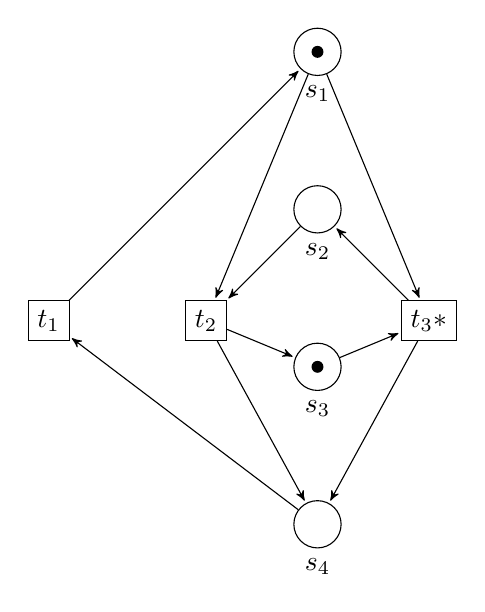
\begin{tikzpicture}[node distance=2cm,>=stealth',bend angle=45,auto]

  					\tikzstyle{place}=[circle,draw=black,minimum size=6mm]
		  			\tikzstyle{transition}=[rectangle,draw=black,minimum size=4mm]

    				\node [place,tokens=1,label=below:$s_1$] (s1) {};
    				\node [place,label=below:$s_2$] (s2) [below of=s1] {};
		    		\node [place,tokens=1,label=below:$s_3$] (s3) [below of=s2] {};
    				\node [place,label=below:$s_4$] (s4) [below of=s3] {};

    				\node [transition] (t2) [below left of=s2] {$t_2$}
		      			edge [pre]  (s1)
      					edge [pre]  (s2)
      					edge [post] (s3)
		      			edge [post] (s4);

    				\node [transition] (t1) [left of=t2] {$t_1$}
      					edge [pre]  (s4)
		      			edge [post] (s1);

    				\node [transition] (t3) [below right of=s2] {$t_3*$}
      					edge [pre]  (s1)
		      			edge [pre]  (s3)
      					edge [post] (s2)
      					edge [post] (s4);
				\end{tikzpicture}
				\hspace{1cm}
		    	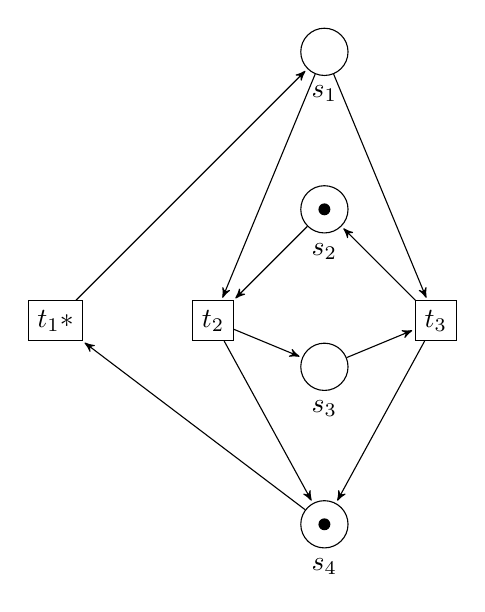
\begin{tikzpicture}[node distance=2cm,>=stealth',bend angle=45,auto]

  					\tikzstyle{place}=[circle,draw=black,minimum size=6mm]
  					\tikzstyle{transition}=[rectangle,draw=black,minimum size=4mm]

		    		\node [place,label=below:$s_1$] (s1) {};
    				\node [place,tokens=1,label=below:$s_2$] (s2) [below of=s1] {};
    				\node [place,label=below:$s_3$] (s3) [below of=s2] {};
		    		\node [place,tokens=1,label=below:$s_4$] (s4) [below of=s3] {};

    				\node [transition] (t2) [below left of=s2] {$t_2$}
      					edge [pre]  (s1)
		      			edge [pre]  (s2)
      					edge [post] (s3)
      					edge [post] (s4);

		    		\node [transition] (t1) [left of=t2] {$t_1*$}
      					edge [pre]  (s4)
      					edge [post] (s1);

		    		\node [transition] (t3) [below right of=s2] {$t_3$}
      					edge [pre]  (s1)
      					edge [pre]  (s3)
		      			edge [post] (s2)
      					edge [post] (s4);
				\end{tikzpicture}
    			\caption{The next two markings ($M_3$ on the left and $M_4$ on the right).}
		    	\label{fig2}
    		\end{figure}
    	\item
    \end{enumerate}

\end{document}
